\documentclass[final]{siamltex}
\input{myhead}

\title{A parallel matrix-free framework for frequency-domain seismic modelling, imaging and
 inversion in Matlab}
\author{Tristan van Leeuwen 
\thanks{Dept. of Earth and Ocean sciences, University of British Columbia, 6339 stores road, Vancouver, BC, Canada, V6T 1Z4
({\tt tleeuwen@eos.ubc.ca})}}
\begin{document}

\maketitle

\begin{abstract}
I present a parallel matrix-free framework for frequency-domain
seismic modeling, imaging and inversion. The framework provides basic building blocks 
for designing and testing optimization-based formulations of both linear and non-linear 
seismic inverse problems.
By overloading standard linear-algebra operations, such as matrix-vector
multiplications, standard optimization packages can be used to work with the code
without any modification. This leads to a scalable testbed on
which new methods can be rapidly prototyped and tested on medium-sized 2D problems. 
I present some numerical examples on both linear and non-linear seismic inverse problems. 
\end{abstract}

\begin{keywords}
Seismic imaging, inverse problems, optimization, Matlab, object-oriented programming
\end{keywords}

\section{Introduction}
Seismic data are a rich source of information on the subsurface. Large amounts
of data are acquired for both academic and industrial purposes,
either through active experiments or by recording earth-quake responses.
Inversion of such data to obtain estimates of subsurface properties, such as soundspeed and density,
is an active area of research both in the geophysics and scientific computing communities 
\cite{virieux09,Symes2009,Epanomeritakis2008}.

A seismic inversion framework needs to combine a modeling engine to solve a wave-equation (e.g., finite
differences or finite elements), (non-) linear optimization algorithms and
facilitate i/o of large amounts of data and the corresponding meta data.
Due to the large scale of typical problems, a computer code that
implements these algorithms has to be extremely efficient, scalable and robust.
On the other hand, the interdisciplinary nature of such projects requires that
experts from different fields contribute to the code. 
Needless to say, some form of unit-testing needs to be incorporated to facilitate de-bugging.
The challenge is in meeting these, seemingly mutually exclusive, requirements.

A necessary (but not sufficient) condition is that the basic
building blocks of the code, such as the modeling operator, its Jacobian and
their basic operations (forward modeling, action of the Jacobian and its
adjoint) are exposed. This allows the units to be tested separately and re-used
for different purposes. Then, these building blocks should be cast in
pre-defined classes, such as (non-) linear operators and functionals.
This allows us to have our code reflect the underlying
mathematical principles and serves a bridge to existing code. 
We do not have to sacrifice efficiency when following
these principles because the individual blocks can still contain highly
optimized code.

An added bonus of such a framework is that it allows for rapid prototyping and
increases reproducibility. Because the separate building blocks
expose the underlying mathematics, it should be relatively straightforward to
understand and implement the algorithm using a different modeling kernel
(given that is also exposes the basic functionality as described above).
Unit tests can ensure that any given implementation is correct.

For further reading on this design philosophy I refer the reader to
\cite{claerbout2012,Symes2011}.
A few existing libraries that facilitate such approaches to various degrees are PETSC 
\cite{petsc}, Trilinos
\cite{Heroux2005}, the Rice Vector Library \cite{Padula2009} and SPOT
\cite{spot}.

\subsection{Framework}
Following the design principles sketched above, I present a 
\emph{parallel} \emph{matrix-free} framework for frequency-domain wavefield modelling, 
imaging and inversion in Matlab. This framework is useful for testing and developing new algorithms to solve
the seismic inverse problem and for educational purposes.

The basic building blocks of the framework
are the finite-difference modeling operator $\mbf{d} = \msf{F}(\mbf{m})$ that maps a model of the subsurface
$\mbf{m}$ to the observed data $\mbf{d}$, and its Jacobian $\nabla\msf{F}(\mbf{m})$, implemented
as matrix-free linear operator. Using these building blocks, we can formulate algorithms to
solve the basic inverse problem
\vspace*{5mm}
\begin{center}
\parbox[c]{.8\textwidth}{
\textit{for given observations $\mbf{d}_{\mathrm{obs}}$, find a model $\mbf{m}$ for which 
the predicted data $F(\mbf{m})$ best fits the observed data.}
}
\end{center}
\vspace*{5mm}

\noindent
In particular, I will focus on optimization-based formulations of this problem
\bq
\min_{\mbf{m}} W(\msf{F}(\mbf{m}),\mbf{d}_{\mathrm{obs}}),
\eq
where $W$ measures the misfit between the observed and predicted data 
(e.g., for non-linear least-squares $W(\cdot,\cdot) = ||\cdot - \cdot||_2^2$).

\subsection{Matlab code}
The Matlab code is available for academic purposes.
The code to reproduce the examples presented in this paper is also included. 
See \url{https://www.slim.eos.ubc.ca/releases} for download instructions.

\subsection{Outline}
First, I discuss the modeling kernel, which consists of the forward modeling
operator and its Jacobian. Then I show how to use a framework for matrix-free
linear algebra in Matlab to implement functionality needed for various imaging and inversion purposes. 
I discuss how the different units of code should be tested and finally, give
some numerical examples on both linear and non-linear seismic inverse problems.

\subsection{Notation}
Throughout the paper I will use the following notation:
\begin{itemize}
\item $x$ - lowercase, italic symbols denote scalars
\item $\mbf{x}$ - lowercase, boldface symbols denotes column vectors whose elements are 
denoted as $x_i$
\item $A$ - capital italic symbols denote matrices or linear operators and
$\transp{\cdot}$ denotes their (conjugate) transpose or adjoint.
%\item we denote stacks and dictionaries as
%\bq
%\mbf{A} &=& \dictt(\{A_k\}_{k=1}^{n}) = (A_1, A_2, \ldots, A_k),\\
%\mbf{A} &=& \stackt(\{A_k\}_{k=1}^{n}) = 
%\left(\begin{array}{c}
%A_1\\
%A_2\\
%\vdots\\
%A_n
%\end{array}\right)\\
%\mbf{A} &=& \blkdt(\{A_k\}_{k=1}^{n}) = 
%\left(\begin{array}{cccc}
%A_1&&&\\
%&A_2&&\\
%&&\ddots&\\
%&&&A_n
%\end{array}\right)
%\eq
\item $\vect(\cdot)$ denotes vectorization, $\vect^{-1}(\cdot)$ denotes reshaping into the
 original size.
\item $\diag(\cdot)$ when applied to a matrix extracts the diagonal from a matrix, when 
applied to a vector constructs a diagonal matrix.
\item $\msf{F}(\cdot)$ - capital sans-serif symbols denote non-linear operators,
and $\nabla\msf{F}$ denotes the Jacobian.
\item $\msf{f}(\cdot)$ - lower case sans-serif symbols denote functions and
$\nabla\msf{f}$ denotes the gradient.
\item $\mcl{S}$ - curly capital letters denote sets/lattices/grids.
\end{itemize}


\section{Modeling}
Wave-propagation in the earth is assumed to obey a scalar Helmholtz equation:
\bq
\label{eq:helmholtz}
A_{\omega}(\mbf{m})\mbf{u} = \mbf{q}.
\eq
Here $A_{\omega}(\mbf{m})$ is the discretized Helmholtz operator
$\omega^2\mbf{m} + \nabla^2$ -- with
some form of absorbing boundary conditions to emulate an infinite domain -- for frequency 
$\omega$ and squared slowness $\mbf{m}$ in seconds$^2$/meters$^2$, $\mbf{u}$ is the wavefield and
$\mbf{q}$ represents the source.

\subsection{Grids}

I define 4 distinct grids that are used during the computations:
\begin{itemize}
\item The physical grid $\mcl{G}$. This grid represents the region of interest.
The medium paramerer $\mbf{m}$ is discretized on this grid.
\item The computational grid $\mcl{C}$, which is an extension of the physical
grid. The Helmholtz operator is discretized on this grid. The extended area is used for
the absorbing boundary conditions.
\item The source grid $\mcl{S}$. This grid is a subset of the physical grid and
is used to define the source functions.
\item The receiver grid $\mcl{R}$. This grid is a subset of the physical grid
and is used to define the receiver array.
\end{itemize}

Figure \ref{fig:grids} illustrates the different grids. Quantities are mapped from one 
grid to the other via interpolation or padding (and their adjoints):
\begin{itemize}
\item $P_{\mcl{X}}$ is a 2D interpolation operator that interpolates from
$\mcl{C}$ to $\mcl{X}$,
\item $E_{\mcl{X}}$ padds the input, defined on grid $\mcl{X}$ with its boundary
 values to the computational grid $\mcl{C}$.
\end{itemize}

\subsection{Source representation}

I use adjoint interpolation to represent point-sources. This ensures that the
point-source will behave like a discretized delta function to some extent.
Consider the following 1D example. The source-grid is a single point $\mcl{S} =
\{ \frac{1}{2}\}$ while the computational grid is given by $\mcl{C} = \{0,
\frac{1}{5}, \frac{2}{5}, \frac{3}{5}, \frac{4}{5}, 1\}$. Define the
interpolation operator $P_{\mcl{S}}$ to interpolate from $\mcl{C}$ to $\mcl{S}$.
The source function on the source grid is a single scalar $\mbf{q} = 1$. The
resulting source functions for linear, quadratic and cubic interpolation are
shown in figure \ref{fig:source}.
For given polynomials $\mbf{p}^{l}=[0,
\frac{1}{5}, \frac{2}{5}, \frac{3}{5}, \frac{4}{5}, 1]^{l}$, we want our discretized delta
 function to satisfy
\bq
\langle \mbf{p}_{l}, \transp{P_{\mcl{S}}}\mbf{q}\rangle_{\mcl{C}} &=&
\left(\ts{\frac{1}{2}}\right)^{l},
\eq
up to some order. We can write this requirement as $\langle
P_{\mcl{C}}\mbf{p}^{l},\mbf{q}\rangle_{\mcl{S}} = P_{\mcl{C}}\mbf{p}^{l} =
(\frac{1}{2})^{l}$, from which it follows that the order to which this
requirement will be satisfied is determined by the accuracy of the interpolation
operator. A numerical verification is shown in table \ref{table:source}.

\subsection{Modeling operator and its Jacobian}
The data for one frequency and source is obtained via
\bq
\mbf{d}_{ij} =
P_{\mcl{R}}A_{\omega_i}(E_{\mcl{G}}\mbf{m})^{-1}\transp{P_{\mcl{S}}}\mbf{q}_{ij}.
\label{eq:F}
\eq
The modeling operator $\msf{F}$ solves (\ref{eq:F}) for several
frequencies $i = 1, \ldots, n_f$ and sources $j = 1,\ldots,n_s$ and organizes the result
in a vector.

The Jacobian of the modeling operator, $\nabla\msf{F}$, for one source and frequency is
given by 
\bq
\frac{\partial \mbf{d}_{ij}}{\partial \mbf{m}} =
P_{\mcl{R}}A_{\omega_i}(E_{\mcl{G}}\mbf{m})^{-1}G_{\omega_i}(\mbf{m},\mbf{u}_{ij})E_{\mcl{G}},
\eq
where $\mbf{u}_{ij} =
A_{\omega_i}(E_{\mcl{G}}\mbf{m})^{-1}\transp{P_{\mcl{S}}}\mbf{q}_{ij}$ and
$G_{\omega}(\mbf{m},\mbf{u}) = \left(\frac{\partial A_{\omega}\mbf{u}}{\partial
\mbf{m}}\right)$.
In practice, the Jacobian matrix is never formed explicitly. Instead, its action is 
computed by solving 2 Helmholtz systems per source and frequency.

\subsection{Analytic solutions}
For some specific cases, analytic expressions exist for the Greens function.
For a constant medium with velocity $c_0$ and a point-source at $(z_s,x_s)$, we have
\bq
\mbf{u} = \frac{\imath}{4}H_{0}^{1}(\omega \mbf{r}/c_0),
\eq
where $H_0^1$ is a Hankel function of the first kind and $r_i = \sqrt{(x_i - x_s)^2 + (z_i - z_s)^2}$.

For linearly increasing velocity $c_0 + \alpha z$ and a point-source at $(z_s,x_s)$, the analytic solution is given by \cite{Kuvshinov2006}
\bq
\mbf{u} = Q_{\nu-\frac{1}{2}}(\mbf{s}),
\eq
where $Q_{\mu}$ is a Legendre function with $\nu = \imath\sqrt{(\omega/\alpha)^2 - \frac{1}{4}}$ and
\[
s_i = 1 + \frac{1}{2}\frac{r_i^2}{(z_s+c_0/\alpha)(z_i+c_0/\alpha)}. 
\]

\section{Matrix-free framework}
The (linearized) modeling operator is readily implemented in Matlab, but
interaction with existing code, especially for linear operators, is not always
straightforward. To facilitate incorporation of these blocks into exisisting
code, I adopt the SPOT toolbox for matrix-free linear algebra \cite{spot}. This allows
us, for example, to perform matrix-free matrix-vector products by overloading the Matlab 
multiplication operation. Furthermore, by insisting on a certain structure of
our non-linear operators we can easily adopt ideas form algorithmic
differentiation to calculate derivatives of combinations of such operators.

\subsection{Linear operators}
To illustrate the workings of SPOT, let us consider the Fourier transform. The following
code fragment defines an operator that performs the Fourier transform on a vector of length
1000 and performs a forward and inverse FFT on a random vector.
\begin{lstlisting}
n = 1000;        % length
A = opDFT(n);    % define SPOT operator
x = randn(n,1);  % random vector of length n
y = A*x;         % forward FFT
x = A'*y;        % inverse/adjoint FFT
\end{lstlisting}
Upon multiplying the operator \texttt{A} with the vector \texttt{x}, Matlab
will call the function \texttt{A.multiply(x,1)}, wich in turn will perform the
Fourier transform using the Matlab built-in function \texttt{fft}. Similarly, when
multiplying the adjoint with \texttt{y}, Matlab will call the function
\texttt{A.multiply(x,-1)}, which in turn calls \texttt{ifft}.

Custom linear operators can be implemented in a similar manner by supplying a
function that performs forward and adjoint multiplication. This function can be directly
wrapped into a standard SPOT operator using \texttt{opFunction}, or the user can define
a custom SPOT operator using the \texttt{opSpot} class. The latter allows one to overload
other Matlab built-in functions, such as \texttt{mldivide}, \texttt{mrdivide}, \texttt{display}, \texttt{norm} etc. Composition and addition of operators is also supported. 
For example, \texttt{C  = A*B}, where \texttt{A} and \texttt{B} are SPOT operators, will return a spot 
operator that multiplies with \texttt{B} and subsequently with \texttt{A}. 
The Kronecker product is supported via \texttt{C = opKron(A,B)}. 
A parallel extension of SPOT, pSPOT \cite{pspot,pacteau} allows us to define linear 
operators that  work on distributed arrays. 

The linear operators can be tested for consistency via the \emph{dot-test}
\bq
\langle A\mbf{x},\mbf{y}\rangle = \langle \mbf{x},\transp{A}\mbf{y}\rangle,
\label{eq:dottest}
\eq
where $\mbf{y}$ has to be in the range of $A$. Typically, one takes $\mbf{x}$ to
be a random vector and we can generate $\mbf{y}$ by acting on another random
vector with $A$. The two should be the same up to numerical precision.

\subsection{Non-linear operators}
For non-linear operators and functions I use the convention that they return
their output (vector or scalar) and the Jacobian or gradient.
This structure makes it extremely easy to implement complictated chains of such
operations. Furthermore, individual components can be tested seperately to
facilitate debugging. One
popular way of testing gradients is based on the Taylor series
\bq
\msf{f}(\mbf{x}_0 + h\delta\mbf{x}) = \msf{f}(\mbf{x}_0) + 
h\langle\nabla\msf{f}(\mbf{x}_0),\delta\mbf{x}\rangle + \mcl{O}(h^2),
\eq
where $\mbf{x}_0$ and $\delta\mbf{x}$ are suitable testvectors. Alternatively, 
we can use the Taylor series at two different points
\bq
\msf{f}(\mbf{x}_2) - \msf{f}(\mbf{x}_1) \approx
\frac{1}{2}\langle \nabla\msf{f}(\mbf{x}_1) + \nabla\msf{f}(\mbf{x}_2), \mbf{x}_2 - \mbf{x}_1\rangle
\eq
Simimarly, for the non-linear operators we have
\bq
\msf{F}(\mbf{x}_0+h\delta\mbf{x}) = \msf{F}(\mbf{x}_0) +
h\nabla\msf{F}(\mbf{x}_1)\delta\mbf{x} + \mcl{O}(h^2).
\label{eq:taylor_jac}
\eq
It is easily verified that the error decays with $h$ as predicted.

\section{Implementation and testing}
The modeling operator is implemented as a Matlab function \texttt{[d,J] = F(m,Q,model)},
where each column of the matrix \texttt{Q} represents a gridded source function,
\texttt{model} is a struct that contains descriptions of the grids and
specifies the frequencies. The output is
the data \texttt{d} and the Jacobian as a SPOT operator \texttt{J}, which
calls the function \texttt{DF(m,Q,input,flag,model)} to compute
the forward (\texttt{flag=1}) or adjoint (\texttt{flag=-1}) action of the Jacobian on 
the vector \texttt{input}.

I use a 9-point mixed-grid stencil \cite{Jo1996} to discretize the Helmholtz operator and use
a sponge boundary condition. The resulting sparse matrix is inverted for all
right-hand-sides simultaneously using Matlab's \texttt{mldivide}, 
which (for sparse matrices) is based on an LU decomposition. 
The loop over frequencies is done in parallel using the Parallel Computing Toolbox, 
as will be discussed later.

Other building blocks, like interpolation, basic i/o and optimization methods
are part of the package. A brief description can be found in the appendix.

\subsection{Accuracy of the modeling code}
The modeling operator is tested against analytic solutions for constant and
linearly increasing velocity profiles $v = v_0 + \alpha z$. Figure
\ref{fig:modeling} (a) shows the error for $v_0=2000$ m/s, $\alpha = 0$ 1/s and
a frequency of 10 Hz as a function of the gridspacing. A slice through the
wavefield is shown in figure \ref{fig:modeling} (b). The analytical and
numerical soltions for $v_0 = 2000$ m/s, $\alpha  = 0.7$ 1/s and a frequency of
10 Hz is shown in figures \ref{fig:modeling} (c) and (d) respectively.

\subsection{Accuracy of the Jacobian}
The accuracy of the Jacobian is tested according to (\ref{eq:taylor_jac}) for a
constant velocity and a random perturbation. The resulting error is shown in
figure \ref{fig:jacobian}.

\subsection{Consistency of the Jacobian}
The consistency of the Jacobian is tested with the dottest (cf. eq.
\ref{eq:dottest}). The result on 10 random vectors is shown in table
\ref{table:adjoint}.

\subsection{Scalability}
The modelling code is parallelized over frequencies using Matlab's Parallel Computing Toolbox.
We use the \emph{Single Program Multiple Data} (SPMD) functionality of this tool
box to divide the computation over the available processors. 
The basic algorithm is as follows:
\begin{lstlisting}
% distribute frequencies using standard distribution
freq = distributed(model.freq);
spmd
	% define distribution of data array
	codistr  = codistributor1d(2,[],[nsrc*nrec,nfreq]);
	% get local frequencies
	freqloc  = getLocalPart(freq);
	nfreqloc = length(freqloc);
    % loop over local frequencies
	for k = 1:nfreqloc
		% solve Helmholtz equation for local frequencies and store resulting data in Dloc
    end
    % build distributed array from local parts
    D = codistributed.build(Dloc,codistr); 
end

\end{lstlisting}

To test the performance of the parallelization, I compute data for a model 
of size 1200 $\times$ 404, for 10 sources and 64 frequencies. 
The compute cluster consists of 36 IBM x3550 nodes, each with 2 quad core Intel 2.6Ghz
CPUs, 16 GB RAM and a Volterra x4 inter-processor network. We used 1 processor
per node plus one master node (used by Matlab to manage the computation and not counted in the 
total number of CPUs used). The results for various numbers of CPUs are shown in table \ref{table:scale}. 


\section{Examples}
\subsection{Seismic Waveform Inversion}
Waveform inversion is a procedure to obtain gridded medium parameters from
seimic data by solving a non-linear data-fitting problem of the form
\bq
\min_{\mbf{m}} \msf{w}\left(\msf{F}(\mbf{m}) - \mbf{d}\right),
\eq
where $\msf{w}$ is some differentiable penalty function. While the classical
formulation of this problem for seismic applications uses a least-squares
penalty \cite{tarantola82}, many other penalties have been proposed in this context.

A standard
optimization-procedure relies on iterative updating of the model:
\bq
\mbf{m}_{k+1} = \mbf{m}_k + \alpha_k\mbf{s}_k,
\eq
where the search direction $\mbf{s}_k$ is obtained from the gradient of the
objective
\bq
\nabla\msf{f}(\mbf{m}_k) =
\transp{\nabla\msf{F}(\mbf{m}_k)}\nabla\msf{w}\left(\msf{F}(\mbf{m}_k) - \mbf{d} \right)
\eq
in some way (e.g., Gauss-Newton, Quasi-Newton or CG).

The least-squares penalty is be implemented as

\begin{lstlisting}
function [f,g] = w_ls(r);
  f = .5*norm(r)^2; % two-norm of residual
  g = r;            % gradient
end
\end{lstlisting}
The least-squares misfit of the form
\[
\msf{f_{LS}}(\mbf{m}) = \frac{1}{2}||\msf{F}(\mbf{m}) - \mbf{d}||_2^2,
\]
is then implemented as
\begin{lstlisting}
function [val,grad] = f_ls(m,Q,dt,model);
  [d,DF]    = F(m,Q,model); % predicted data
  r         = d - dt;       % residual
  [val,df]  = w_ls(r);      % penalty
  grad      = DF'*df;       % gradient
end
\end{lstlisting}

This function can be passed on to any black-box optimization method that uses
only function-values and gradients. A Gauss-Newton method can be easily implemented by
having the function return the Gauss-Newton Hessian as SPOT operator.

To illustrate the approach we use the BG Compass velocity model depicted in figure \ref{fig:fwi1} (a). 
We generate data for this model for 71 sources and 281 receivers, 
all equi-spaced and located at the top of the model.  For the inversion we use a
\emph{multi-scale} strategy \cite{sirgue03}, inverting the data in consecutive frequency bands
$f_1 = \{2.5, 3, 3.5\}, f_2 = \{5.5, 6, 6.5\}, f_3 =\{11.5, 12, 12.5\} , f_4 = \{17.5, 18, 18.5\}$, each time using the end result as
initial guess for the next frequency band. The initial model for the first frequency band 
is depicted in figure \ref{fig:fwi1} (b). We use 10 L-BFGS iterations for each frequency band. The 
results are depicted in figure \ref{fig:fwi2}.

\subsection{Reverse time migration}
A seismic image can be obtained from reflection data via backpropagation
\bq
\delta\mbf{m} = \transp{\nabla\msf{F}}\delta\mbf{d}.
\eq
This is referred to as \emph{reverse-time migration} in the geophysical literature. 
The fact that this simple backprojection yields a useable image at all is due to the
fact that the Normal operator $\transp{\nabla\msf{F}}\nabla\msf{F}$ acts as local
scaling and filtering operation only \cite{symes08a}. Many approaches have been developed to estimate
the inverse of this filter without explicitly inverting the normal operator. Following 
\cite{herrmann2008} we estimate the image as
\bq
\delta\mbf{m} = W_{\mbf{x}}\transp{\nabla\msf{F}}W_{\omega}\mbf{d},
\eq
where $W_{\mbf{x}}$ represents the spatial weighting and $W_{\omega}$ represents
a frequency-weighting with $|\omega|^{-1}$. Herrmann et al. \cite{herrmann2008} take $W_{\mbf{x}}$ to be a 
diagonal weighting in the Curvelet domain. For the sake of this example, however, we use
a simple spatial weighting with $\sqrt{z})$ to correct for the geometric spreading.

The following code implements this procedure:

\begin{lstlisting}
% reverse time migration for given data d and background model m0

% get data and Jacobian
[d0,DF] = F(m0,Q,model);

% weighting with |\omega|^{-1}
Wf = oppKron2Lo(opDiag(1./freq),opDirac(nsrc*nrec));

% depth weighting
Wz = opKron(opDirac(n(2)),opDiag(sqrt(z)));

% reverse-time migration
dm = Wz*DF'*(Wf*(d - d0));

\end{lstlisting}

Note the use of the parallel Kronecker product \texttt{oppKron2Lo} which works on arrays that
are distributed along the last dimension (frequency, in this case). To avoid artifacts due 
to non-reflected events in the data, I subtract data for the background model. I illustrate
the algorithm on the Marmousi model, depicted in figure \ref{fig:rtm} (a), using 101 sources, 201 receivers 
(equispaced at the top of the model) and frequencies between 2.5 and 20 Hz with 0.5 Hz increments. 
The background model, depicted in figure \ref{fig:rtm} (b), is a smooth version of this model.
The true perturbation (i.e., the difference between the true
and background model) is shown in figure \ref{fig:rtm} (c). The resulting image is shown in
figure \ref{fig:rtm} (d).

\subsection{Seismic tomography}
Tomographic inversion relies on traveltime information to invert for the velocity. 
Traditionally, traveltimes are manually picked from the data and predicted traveltimes
are computed using a geometric-optics approximating as is also used x-ray tomography. 
The last two decades there has been an increasing interest in generalizing this approach
to finite-frequency regime where wave propagation is no longer accurately modeled via rays.
One way to define the \emph{finite-frequency} traveltime is to consider the correlation of the observed data
with the data for some reference model, and pick the maximum \cite{Luo1991}. 
The observed traveltime \emph{difference} w.r.t. to the reference model for source $i$ and receiver $j$ is then given by
\bq
\delta t^{\mathrm{obs}}_{ij} = \argmax_{t} \sum_{\omega}\left(d_{ij}(\omega)\right)^*d_{ij}^{\mathrm{obs}}(\omega)
e^{\imath\omega t},
\eq
where $d_{ij}^{\mathrm{obs}}(\omega)$ is the observed data and $d_{ij}(\omega)$ is the 
modeled data for the reference model (i.e., $\mbf{d} = \msf{F}(\mbf{m}_0)$). By correlating
the data for the reference model with predicted data for a model $\mbf{m}$ we can compute
the predicted traveltime difference $\delta \mbf{t}(\mbf{m})$ in a similar manner. The goal
then is to find a model $\mbf{m}$ such that $\delta \mbf{t}(\mbf{m}) \approx \delta\mbf{t}^{\mathrm{obs}}$.
For the purpose of inversion the relation between the traveltime difference and the model 
perturbation $\delta \mbf{m} = \mbf{m} - \mbf{m}_0$ is usually linearized, yielding 
\bq
\delta t_{ij} = \frac{\sum_{\omega} \imath\omega \left(d_{ij}(\omega)\right)^* \delta d_{ij}(\omega)}{\sum_{\omega} \omega^2|d_{ij}(\omega)|^2},
\eq
where $\delta d_{ij}(\omega)$ is the linearized data for 
the model perturbation $\delta\mbf{m}$ (i.e., $\delta \mbf{d} = \nabla\msf{F}(\mbf{m}_0)\delta\mbf{m}$). 
We can write this relation as $\delta\mbf{t} = K\delta\mbf{m}$, where the rows of $K$ are 
the so-called \emph{sensitivity kernels}.
For an in-depth overview and further references we refer to \cite{fichtner10}.

In case of constant reference velocity we can implement the (linearized) scattering operator
using the Greens function:
\bq
\delta \mbf{d}(\omega) = \omega^2 G_r(\omega)\diag(\delta\mbf{m})G_s(\omega),
\eq
where $G_r$ denotes the Greens function from the receivers to the subsurface and $G_s$ denotes
the Greens function from the subsurface to the sources. 
\begin{lstlisting}
function output = Ktomo(v0,input,flag)

% get reference wavefield and scale factor
for k = 1:nfreq
	d_ref(:,:,k) = ... % reference data
	scale = scale + omega(k)^2*abs(d_ref(:,:,k));
end

% input
if flag > 0 
	output = zeros(nrec,nsrc);
else
	input  = reshape(input,[nrec,nsrc])./scale;
	output = zeros(nz*nx,1);
end


for k = 1:nfreq % loop over frequencies
	Gs  = ...   % source wavefield
	Gr  = ...   % receiver wavefield
	
	if flag > 0 % forward mode
		d_scat = omega(k)^2*Gr*diag(input)*Gs;
		output = output + 1i*omega(k)*conj(d_ref(:,:,k)).*d_scat;
	else        % adjoint mode
		input_k = -1i*omega(k)*d_ref(:,:,k).*input;
		output  = output + omega(k)^2*diag(Gr'*input_k*Gs');
	end
end

% output
if flag > 0
	output = vec(output./scale);
end
	
end
\end{lstlisting}

To illustrate the method, I use the velocity model depicted in figure \ref{fig:tomo1} (a).
The data are modeled for frequencies 0.5 Hz to 20 Hz with 0.5 Hz increments and 
21 sources and 21 receivers which are equally distributed along vertical lines on the left 
and right side of the model at $x=10$ and $x=990$ respectively.  As outlined above, 
the traveltime data are obtained by correlating this data with the data for the 
reference model (a constant velocity of 2000 m/s in this case), and picking the maximum value
for each source-receiver pair. The resulting traveltime data is shown in figure \ref{fig:tomo1} (b).
An example of the corresponding waveform data for the true and reference model is shown in figures
\ref{fig:tomo1} (c,d). The correlation panel and the picked traveltimes are shown in figure \ref{fig:tomo1} (c).
The scattering operator is implemented using the analytic expression for the Greens function discussed earlier.
An example of the sensitivity kernel for one source and receiver is shown in figure \ref{fig:tomo2} (a). 
Smoothness is imposed on the solution by representing the model on a coarser grid with cubic splines.
For this example, the spline grid is defined as $\mcl{B}_{x} = \{100, 300, 500, \ldots, 900\}$ and 
$\mcl{B}_{z} = \{100, 200, 300, \ldots, 900\}$. For the the spline evaluation I use \texttt{opSpline1D} with
Dirichlet boundary conditions in the $z$ direction and Neumann boundary conditions in the 
$x$ direction. Matlab's \texttt{lsqr} is used to solve the resulting linear system. 
The results after 10 iterations is shown in figure \ref{fig:tomo2} (b). The code to perform this
experiment is given by 

\begin{lstlisting}
% spline grid
xs = [100:200:900];
zs = [100:100:900];

% spline operators
Bx = opSpline1D(xs,x,[1 1]);
Bz = opSpline2D(zs,z,[0 0]);
B  = opKron(Bx,Bz);

% wrap function Ktomo in SPOT operator
K  = opFunction(...

% call LSQR
dm = lsqr(K*B,T,1e-6,10);

\end{lstlisting}

\section{Conclusion and discussion}
I present a flexible and scalable framework for prototyping algorithms for seismic imaging and inversion
and illustrate it with both linear and non-linear examples.
The code may also be useful for other applications, such as Medical imaging \cite{natterer01}.

The object-oriented approach allows us to design
complicated algorithms from relatively simple, easy to maintain, building blocks. 
Separate pieces of the code can be easily tested, re-used or swapped out. 
For example, we can use a different wave-equation and leave the rest of the code unchanged. 
The use of operator overloading allows us to easily interface with existing optimization codes.

Future work will be aimed at further abstraction of data-structures. Matlab already allows us to
work with distributed arrays with relative ease by taking care of communication automatically.
In a similar fashion, Matlab's \texttt{memmap} functionality can be used to acces 
data that is stored on disk as if it was a Matlab array. Such an approach would allow
us to scale the same algorithms to very large data-sets, for example by adopting Google's
MapReduce model \cite{Dean04}. 

\section*{Acknowledgments}
I thank everybody at the Seismic Laboratory for Imaging and Modeling (SLIM) at UBC 
for their feedback and help with developing this software. 
The BG Compass velocity model was made available by the BG Group.
This work was in part financially supported by the Natural Sciences and 
Engineering Research Council of Canada Discovery Grant (22R81254) and the 
Collaborative Research and Development Grant DNOISE II (375142-08). 
This research was carried out as part of the SINBAD II project with support 
from the following organizations: 
BG Group, BP, Chevron, ConocoPhillips, Petrobras, Total SA, and WesternGeco.


\clearpage
\bibliographystyle{siam}
\bibliography{mybib}
%
\clearpage
\begin{table}[ht]
\centering
\begin{tabular}{cccc}
& linear & quadratic & cubic \\
\hline
0 & 0.000000e+00 & 0.000000e+00 & 0.000000e+00 \\
1 & 0.000000e+00 & 5.551115e-17 & 5.551115e-17 \\
2 & 1.000000e-02 & 0.000000e+00 & 0.000000e+00 \\
3 & 1.500000e-02 & 3.000000e-03 & 0.000000e+00 \\
4 & 1.510000e-02 & 5.100000e-03 & 9.000000e-04 \\
5 & 1.275000e-02 & 5.550000e-03 & 2.250000e-03 \\
\hline
\end{tabular}

\caption{Accuracy of the discretized delta function for $l=0, 1, \ldots, 5$
using linear, quadratic and cubic interpolation.}
\label{table:source}
\end{table}

\begin{table}[ht]
\centering
\begin{tabular}{ccc}
 $\Re\langle A\mbf{x},\mbf{y} \rangle$ & $\Re\langle \mbf{x},A^{\dagger}\mbf{y} \rangle$ & error \\
\hline
2.453000e+07 & 2.453000e+07 & 2.220400e-14 \\
1.762400e+08 & 1.762400e+08 & 3.552700e-15 \\
1.896000e+08 & 1.896000e+08 & 1.421100e-14 \\
-4.902800e+07 & -4.902800e+07 & 7.194200e-14 \\
1.295700e+08 & 1.295700e+08 & 3.197400e-14 \\
-4.529400e+08 & -4.529400e+08 & 3.197400e-14 \\
-1.711600e+08 & -1.711600e+08 & 3.206300e-13 \\
-3.416800e+08 & -3.416800e+08 & 0.000000e+00 \\
-8.159100e+08 & -8.159100e+08 & 1.421100e-14 \\
3.125000e+07 & 3.125000e+07 & 7.993600e-15 \\
\hline
\end{tabular}

\caption{Dot-test of Jacobian on random test vectors.}
\label{table:adjoint}
\end{table}

\begin{table}[ht]
\centering
\begin{tabular}{ccc}
 \# of procs & time [s] & efficiency \\
\hline
1.00 & 2459.00 & 1.00 \\
2.00 & 1224.00 & 1.00 \\
4.00 & 615.00 & 1.00 \\
8.00 & 313.00 & 0.98 \\
16.00 & 188.00 & 0.82 \\
\hline
\end{tabular}

\caption{Scalability test of forward modeling operator on a 1200x404 model for 64 frequencies and 10 sources using different
numbers of CPUs. The times are averages over 5 runs.}
\label{table:scale}
\end{table}

\clearpage
\begin{figure}
\centering
\includegraphics[scale=1]{./figs/grids}
\caption{Illustration of grids used for modeling. The physical grid (white) is
extended on all sides (grey) to define the computational grid. Examples of the
source and receiver grids are also shown.}
\label{fig:grids}
\end{figure}


\begin{figure}[ht]
\centering
\includegraphics[scale=.5]{./figs/source_a}
\caption{Discretization of a delta function $\delta(x-\frac{1}{2})$ using linear, quadratic and cubic
interpolation.}
\label{fig:source}
\end{figure}

\begin{figure}[ht]
\centering
\begin{tabular}{cc}
\includegraphics[scale=.3]{./figs/modeling_a}&
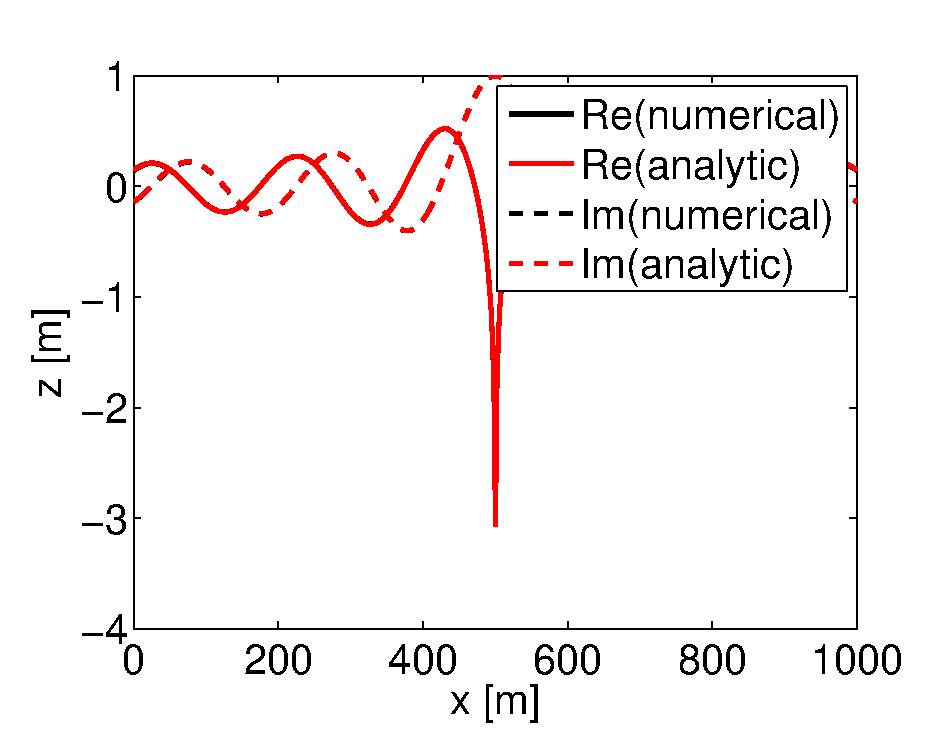
\includegraphics[scale=.3]{./figs/modeling_b}\\
{\small (a)}&{\small (b)}\\
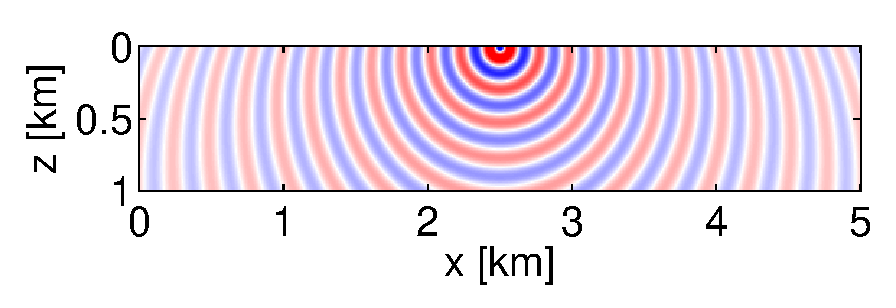
\includegraphics[scale=.3]{./figs/vz_a}&
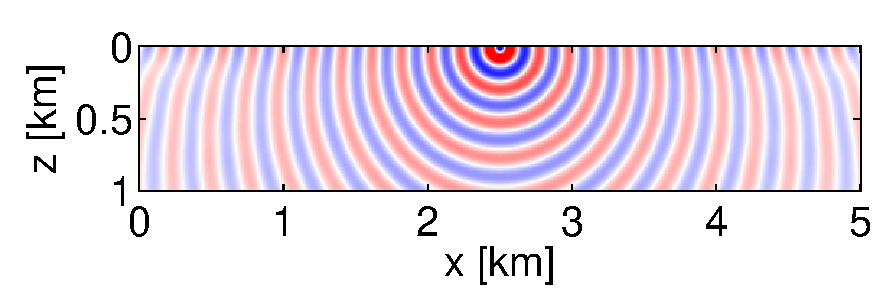
\includegraphics[scale=.3]{./figs/vz_b}\\
{\small (c)}&{\small (d)}\\
\end{tabular}
\caption{Accuracy of the modeling operator. (a) error between analytic and
numerical solution for constant velocity $v_0 = 2000$ m/s and a frequency of 10
Hz. on a domain of 1000 m$\times$ 1000 m with a point source in the center. (b)
Wavefields at $z = 500$m. (c-d) Analytic and numerical solution for linear
velocity profile $2000 + 0.7z$ and a frequency of 10 Hz.}
\label{fig:modeling}
\end{figure}

\begin{figure}[ht]
\centering
\includegraphics[scale=.5]{./figs/error_jacobian_a}
\caption{bla}
\label{fig:jacobian}
\end{figure}

\begin{figure}[ht]
\centering
\begin{tabular}{cc}
\includegraphics[scale=.4]{./figs/fwi_a}&
\includegraphics[scale=.4]{./figs/fwi_b}\\
{\small (a)}&{\small (b)}\\
\end{tabular}
\caption{(a) BG Compass velocity model and (b) initial model for FWI example.}
\label{fig:fwi1}
\end{figure}

\begin{figure}[ht]
\centering
\begin{tabular}{cc}
\includegraphics[scale=.4]{./figs/fwi_c}&
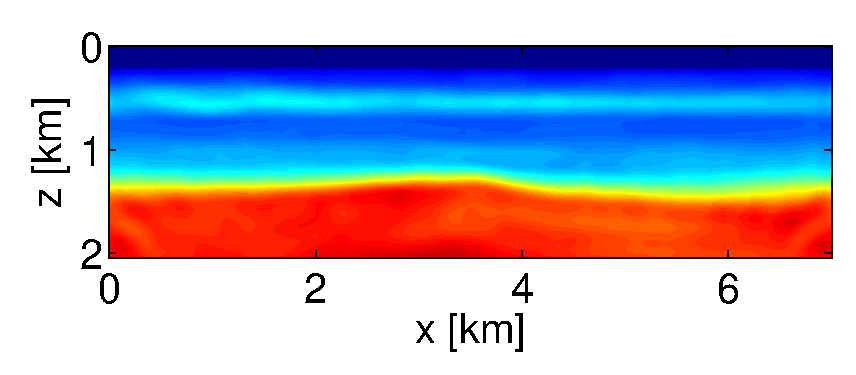
\includegraphics[scale=.4]{./figs/fwi_d}\\
{\small (a)}&{\small (b)}\\
\includegraphics[scale=.4]{./figs/fwi_e}&
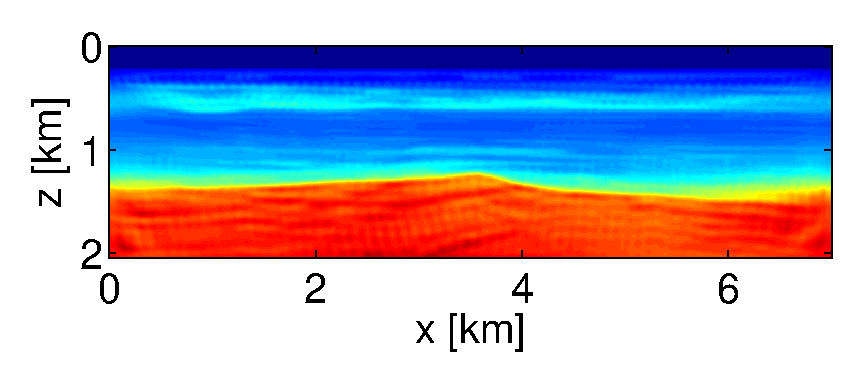
\includegraphics[scale=.4]{./figs/fwi_f}\\
{\small (c)}&{\small (d)}\\
\end{tabular}
\caption{Result of the inversion of subsequent frequency bands: (a) 2.5-3.5 Hz, (b) 5.5-6.5 Hz, (c) 11.5-12.5 Hz and (d) 17.5-18.8 Hz, 
each after 10 L-BFGS iterations using the previous result as starting model.}
\label{fig:fwi2}
\end{figure}

\begin{figure}[ht]
\centering
\begin{tabular}{cc}
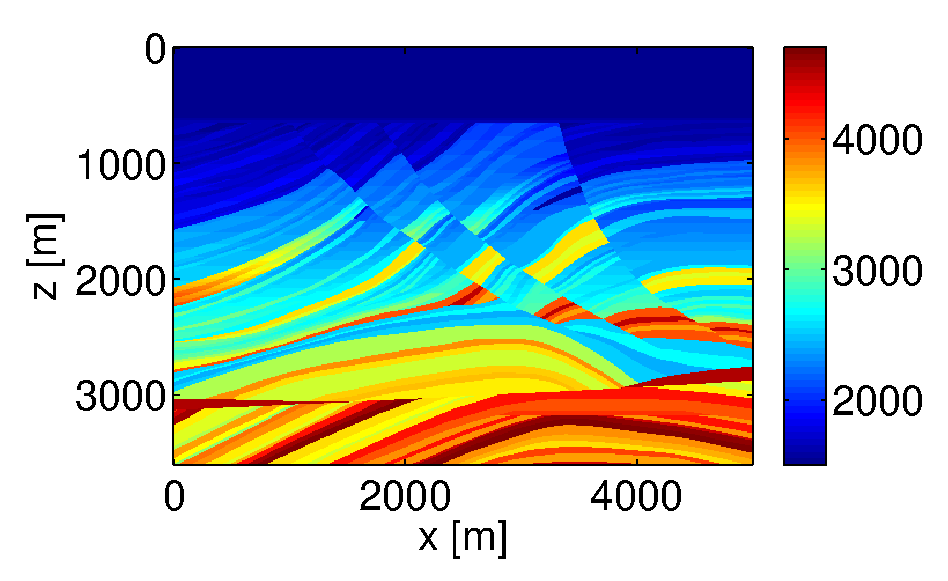
\includegraphics[scale=.4]{./figs/rtm_a}&
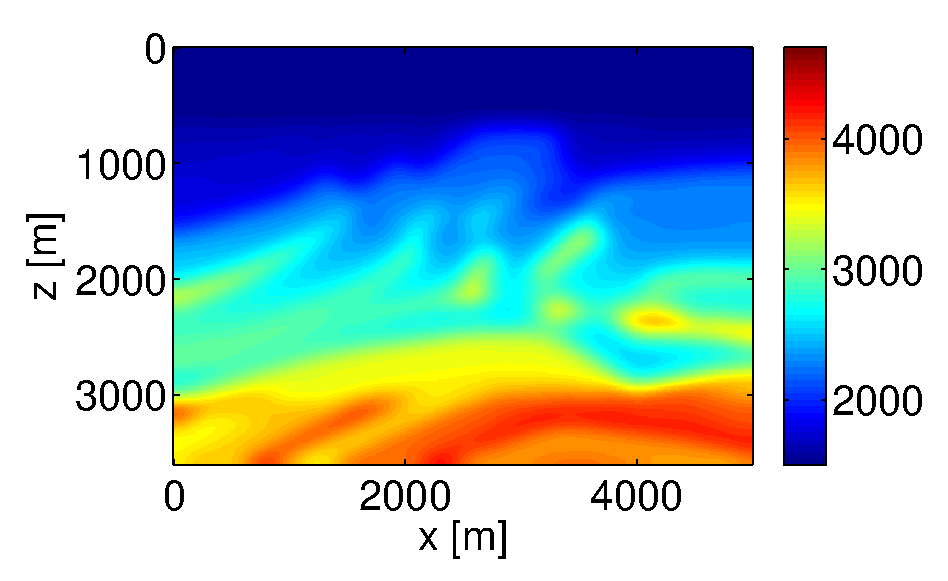
\includegraphics[scale=.4]{./figs/rtm_b}\\
{\small (a)}&{\small (b)}\\
\includegraphics[scale=.35]{./figs/rtm_c}&
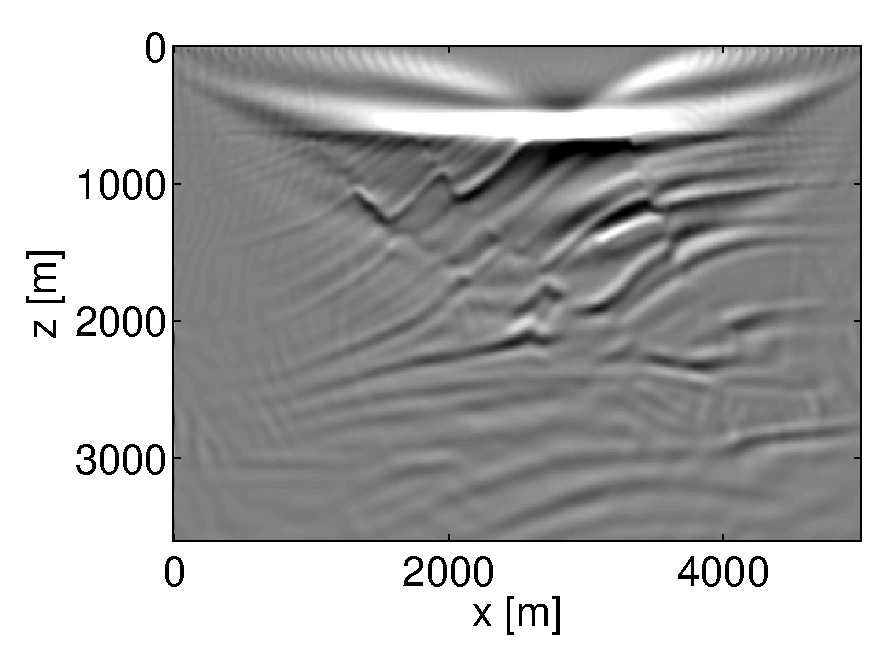
\includegraphics[scale=.35]{./figs/rtm_d}\\
{\small (a)}&{\small (b)}\\
\end{tabular}
\caption{(a) Marmousi velocity model (m/s). (b) Background model used for imaging (m/s). (c) true perturbation.
(d) image.}
\label{fig:rtm}
\end{figure}


\begin{figure}[ht]
\centering
\begin{tabular}{cc}
\includegraphics[scale=.35]{./figs/tomo_f}&
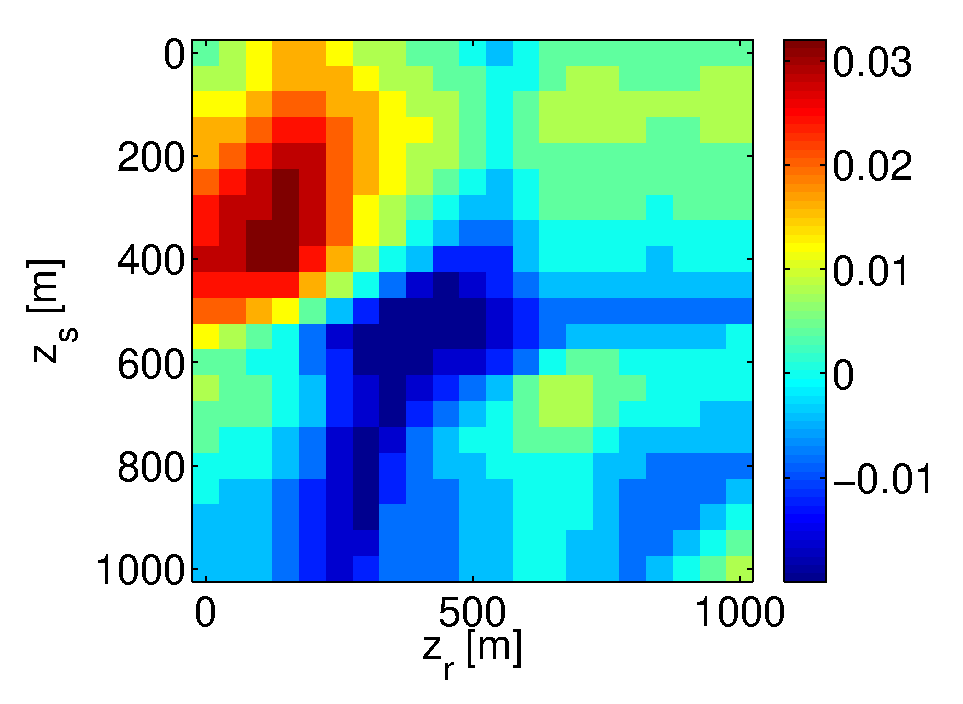
\includegraphics[scale=.35]{./figs/tomo_d}\\
{\small (a)}&{\small (b)}\\
\end{tabular}
\begin{tabular}{ccc}
\includegraphics[scale=.45]{./figs/tomo_a}&
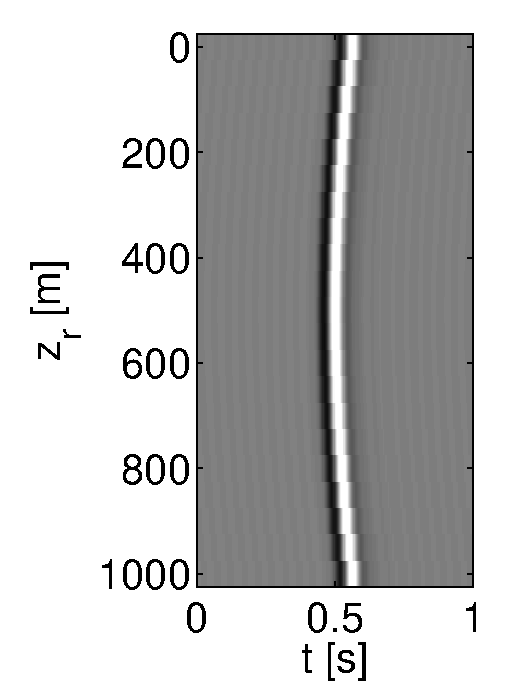
\includegraphics[scale=.45]{./figs/tomo_b}&
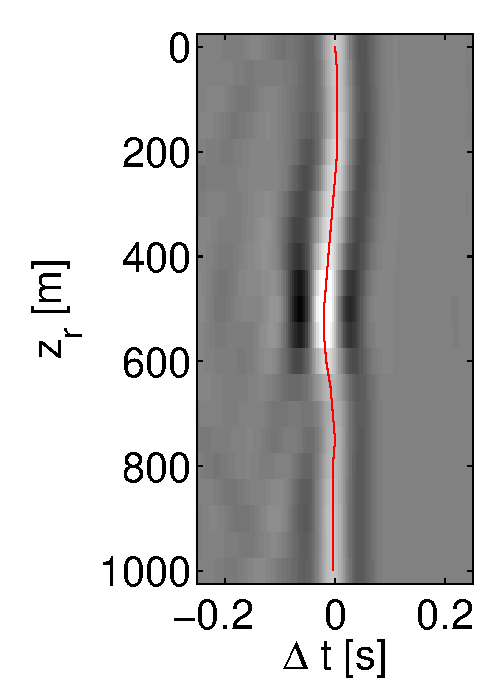
\includegraphics[scale=.45]{./figs/tomo_c}\\
{\small (c)}&{\small (d)}&{\small (e)}\\
\end{tabular}
\caption{The velocity model (m/s) used in tomographic example is shown in (a), the corresponding
traveltime data (s) for each source-receive pair is shown in (b). The waveform data for a source
located at $x=10,z=500$ is depicted in (b); (c) shows the data for the initial homogeneous velocity (2000 m/s) and (d)
shows the correlation of these two and the picked traveltimes.}
\label{fig:tomo1}
\end{figure}

\begin{figure}[ht]
\centering
\begin{tabular}{cc}
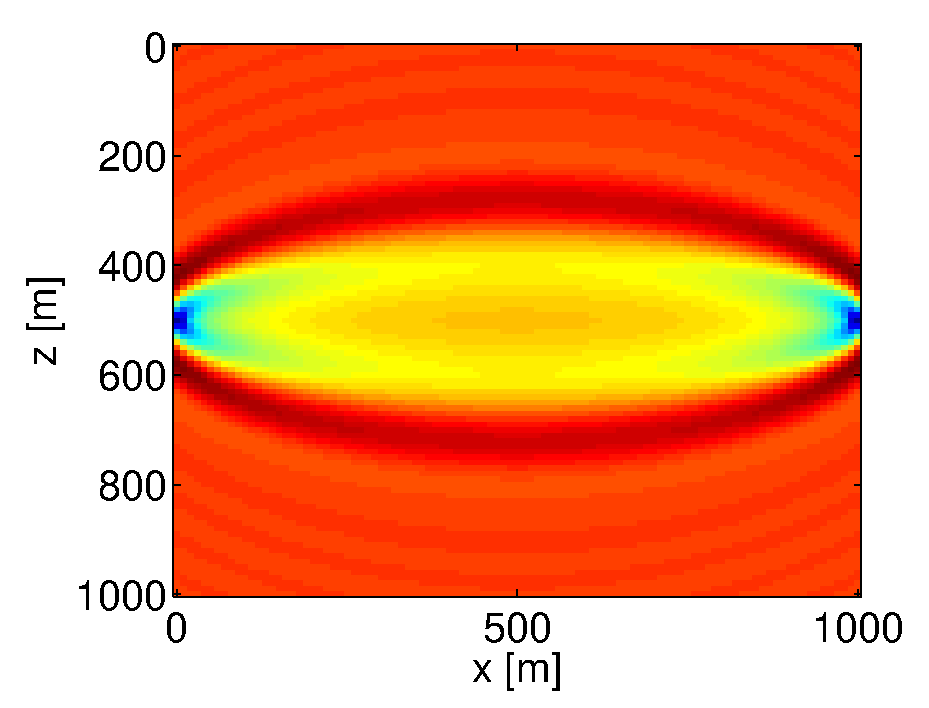
\includegraphics[scale=.35]{./figs/tomo_e}&
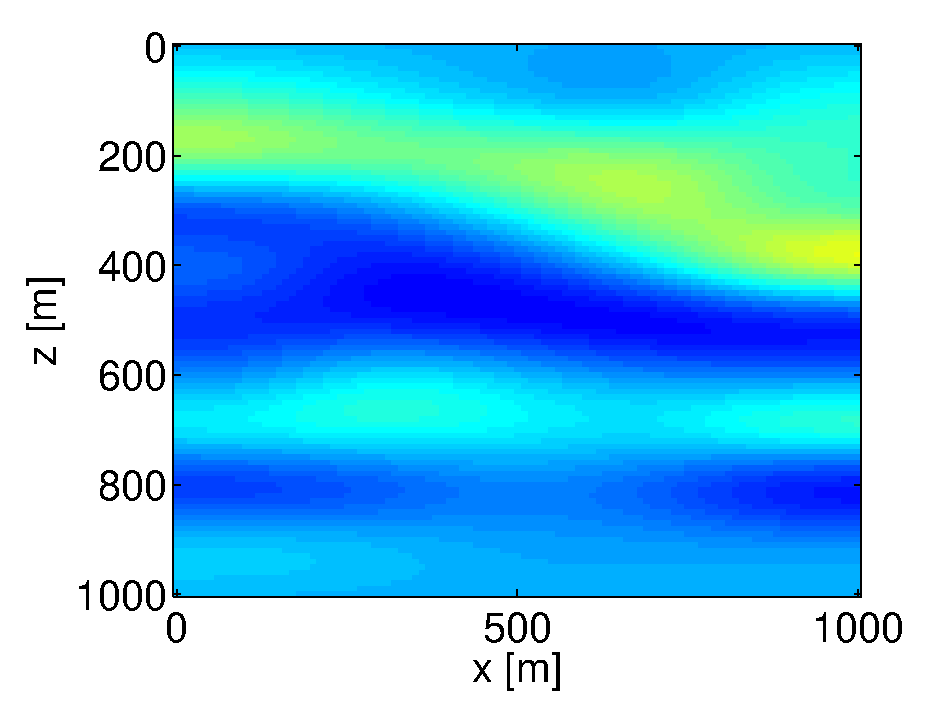
\includegraphics[scale=.35]{./figs/tomo_g}\\
{\small (a)}&{\small (b)}\\
\end{tabular}
\caption{(a) sensitivity kernel for one source-receiver pair. (b) reconstruction after 20 LSQR iterations
 on the same colorscale as figure \ref{fig:tomo1} (a).}
\label{fig:tomo2}
\end{figure}


%\begin{figure}
%\centering
%\includegraphics[scale=.5]{./figs/tomo}
%\caption{Setup for ultrasound example. Plane waves are emitted and the scattered
%wavefield is recorded by an array of receivers that surrounds the object.}
%\label{fig:tomo}
%\end{figure}
%
%\begin{figure}[ht]
%\centering
%\begin{tabular}{ccc}
%\includegraphics[scale=.3]{./figs/ultrasound_a}&
%\includegraphics[scale=.3]{./figs/ultrasound_b}&
%\includegraphics[scale=.3]{./figs/ultrasound_c}\\
%{\small (a)}&{\small (b)}&{\small (c)}\\
%\end{tabular}
%\caption{Ultrasound recovery results. (a) True perturbation, 
%(b) result with 10 iterations of LSMR, (c) result of sparsity promoting formulation.}
%\label{fig:tomo2}
%\end{figure}

\clearpage
\appendix
\section{Matlab Package}
The Matlab code can be downloaded from \url{https://www.slim.eos.ubc.ca/releases}. 
It has been tested with Matlab 2011b. The Parallel Computing Toolbox is needed to take
advantage of the parallelism, though the code will run in serial model without the toolbox as well.

Below is a short description of the contents of the package.
\subsection*{\texttt{tools/utilities/}}
\begin{itemize}
\item{\texttt{SPOT-SLIM} -- SPOT toolbox}
\item{\texttt{pSPOT} -- pSPOT toolbox}
\end{itemize}

\subsection*{\texttt{tools/algorithms/2DFreqModeling/}}
\begin{itemize}
\item{\texttt{F} -- Modelling operator}
\item{\texttt{DF} -- Jacobian of \texttt{F}}
\item{\texttt{oppDF} -- pSPOT constructor of Jacobian, uses \texttt{DF}}
\item{\texttt{G} -- Modelling operator for velocity of the form $v(z) = v_0 + \alpha z$}
\item{\texttt{legendreQ} -- evaluates the Legendre Q function $Q_{\nu}(z)$}
\item{\texttt{Helm2D} -- discretized Helmholtz operator}

\end{itemize}

\subsection*{\texttt{tools/operators/misc/}}
\begin{itemize}
\item{\texttt{opLinterp1D} -- 1D cubic Lagrange interpolation}
\item{\texttt{opLinterp2D} -- 2D linear Lagrange interpolation}
\item{\texttt{opSpline1D} -- 1D Cubic Spline evaluation}
\item{\texttt{opSpline2D} -- 2D Cubic Spline evaluation}
\item{\texttt{opExtension} -- 1D padding}
\item{\texttt{opDFTR} -- Fourier transform for real signals; returns only positive frequencies.}
\end{itemize}

\subsection*{\texttt{tools/functions/misc/}}
\begin{itemize}
\item{\texttt{vec}, \texttt{invvec} -- vectorize (distributed) array 
and reshape (distributed) -- vector back to (distributed) n-dimensional array.}
\item{\texttt{odn2grid, \texttt{grid2odn}} -- convert offset-increment-size
vectors to grid vectors and vice-versa.}
\item{\texttt{odnread}, \texttt{odnwrite} -- read/write for gridded data.}
\end{itemize}


\subsection*{\texttt{tools/solvers/QuasiNewton/}}
\begin{itemize}
\item{\texttt{lbfgs}  -- L-BFGS method with weak Wolfe linesearch}
\end{itemize}

\subsection*{\texttt{applications/SoftwareDemos/2DSMII}}
\begin{itemize}
\item{\texttt{mbin/f\_ls} -- Least-squares misfit and gradient}
\item{\texttt{mbin/w\_ls} -- compute two-norm of vector and its gradient.}
\item{\texttt{mbin/Ktomo} -- Scattering operator for traveltime tomography example}
\item{\texttt{scripts} -- scripts to produce examples}
\item{\texttt{doc}  -- documentation in html format}
\end{itemize}
\end{document}

